
%% bare_conf.tex
%% V1.3
%% 2007/01/11
%% by Michael Shell
%% See:
%% http://www.michaelshell.org/
%% for current contact information.
%%
%% This is a skeleton file demonstrating the use of IEEEtran.cls
%% (requires IEEEtran.cls version 1.7 or later) with an IEEE conference paper.
%%
%% Support sites:
%% http://www.michaelshell.org/tex/ieeetran/
%% http://www.ctan.org/tex-archive/macros/latex/contrib/IEEEtran/
%% and
%% http://www.ieee.org/

%%*************************************************************************
%% Legal Notice:
%% This code is offered as-is without any warranty either expressed or
%% implied; without even the implied warranty of MERCHANTABILITY or
%% FITNESS FOR A PARTICULAR PURPOSE! 
%% User assumes all risk.
%% In no event shall IEEE or any contributor to this code be liable for
%% any damages or losses, including, but not limited to, incidental,
%% consequential, or any other damages, resulting from the use or misuse
%% of any information contained here.
%%
%% All comments are the opinions of their respective authors and are not
%% necessarily endorsed by the IEEE.
%%
%% This work is distributed under the LaTeX Project Public License (LPPL)
%% ( http://www.latex-project.org/ ) version 1.3, and may be freely used,
%% distributed and modified. A copy of the LPPL, version 1.3, is included
%% in the base LaTeX documentation of all distributions of LaTeX released
%% 2003/12/01 or later.
%% Retain all contribution notices and credits.
%% ** Modified files should be clearly indicated as such, including  **
%% ** renaming them and changing author support contact information. **
%%
%% File list of work: IEEEtran.cls, IEEEtran_HOWTO.pdf, bare_adv.tex,
%%                    bare_conf.tex, bare_jrnl.tex, bare_jrnl_compsoc.tex
%%*************************************************************************

% *** Authors should verify (and, if needed, correct) their LaTeX system  ***
% *** with the testflow diagnostic prior to trusting their LaTeX platform ***
% *** with production work. IEEE's font choices can trigger bugs that do  ***
% *** not appear when using other class files.                            ***
% The testflow support page is at:
% http://www.michaelshell.org/tex/testflow/



% Note that the a4paper option is mainly intended so that authors in
% countries using A4 can easily print to A4 and see how their papers will
% look in print - the typesetting of the document will not typically be
% affected with changes in paper size (but the bottom and side margins will).
% Use the testflow package mentioned above to verify correct handling of
% both paper sizes by the user's LaTeX system.
%
% Also note that the "draftcls" or "draftclsnofoot", not "draft", option
% should be used if it is desired that the figures are to be displayed in
% draft mode.
%
\documentclass{IEEEtran4PSCC}
\usepackage{blindtext, graphicx}
\usepackage{soul,color,booktabs,microtype,tabularx}
\usepackage[T1]{fontenc}
\usepackage[utf8]{inputenc}
% Add the compsoc option for Computer Society conferences.
%
% If IEEEtran.cls has not been installed into the LaTeX system files,
% manually specify the path to it like:
% \documentclass[conference]{../sty/IEEEtran}





% Some very useful LaTeX packages include:
% (uncomment the ones you want to load)


% *** MISC UTILITY PACKAGES ***
%
%\usepackage{ifpdf}
% Heiko Oberdiek's ifpdf.sty is very useful if you need conditional
% compilation based on whether the output is pdf or dvi.
% usage:
% \ifpdf
%   % pdf code
% \else
%   % dvi code
% \fi
% The latest version of ifpdf.sty can be obtained from:
% http://www.ctan.org/tex-archive/macros/latex/contrib/oberdiek/
% Also, note that IEEEtran.cls V1.7 and later provides a builtin
% \ifCLASSINFOpdf conditional that works the same way.
% When switching from latex to pdflatex and vice-versa, the compiler may
% have to be run twice to clear warning/error messages.






% *** CITATION PACKAGES ***
%
%\usepackage{cite}
% cite.sty was written by Donald Arseneau
% V1.6 and later of IEEEtran pre-defines the format of the cite.sty package
% \cite{} output to follow that of IEEE. Loading the cite package will
% result in citation numbers being automatically sorted and properly
% "compressed/ranged". e.g., [1], [9], [2], [7], [5], [6] without using
% cite.sty will become [1], [2], [5]--[7], [9] using cite.sty. cite.sty's
% \cite will automatically add leading space, if needed. Use cite.sty's
% noadjust option (cite.sty V3.8 and later) if you want to turn this off.
% cite.sty is already installed on most LaTeX systems. Be sure and use
% version 4.0 (2003-05-27) and later if using hyperref.sty. cite.sty does
% not currently provide for hyperlinked citations.
% The latest version can be obtained at:
% http://www.ctan.org/tex-archive/macros/latex/contrib/cite/
% The documentation is contained in the cite.sty file itself.






% *** GRAPHICS RELATED PACKAGES ***
%
\ifCLASSINFOpdf
  % \usepackage[pdftex]{graphicx}
  % declare the path(s) where your graphic files are
  % \graphicspath{{../pdf/}{../jpeg/}}
  % and their extensions so you won't have to specify these with
  % every instance of \includegraphics
  % \DeclareGraphicsExtensions{.pdf,.jpeg,.png}
\else
  % or other class option (dvipsone, dvipdf, if not using dvips). graphicx
  % will default to the driver specified in the system graphics.cfg if no
  % driver is specified.
  % \usepackage[dvips]{graphicx}
  % declare the path(s) where your graphic files are
  % \graphicspath{{../eps/}}
  % and their extensions so you won't have to specify these with
  % every instance of \includegraphics
  % \DeclareGraphicsExtensions{.eps}
\fi
% graphicx was written by David Carlisle and Sebastian Rahtz. It is
% required if you want graphics, photos, etc. graphicx.sty is already
% installed on most LaTeX systems. The latest version and documentation can
% be obtained at: 
% http://www.ctan.org/tex-archive/macros/latex/required/graphics/
% Another good source of documentation is "Using Imported Graphics in
% LaTeX2e" by Keith Reckdahl which can be found as epslatex.ps or
% epslatex.pdf at: http://www.ctan.org/tex-archive/info/
%
% latex, and pdflatex in dvi mode, support graphics in encapsulated
% postscript (.eps) format. pdflatex in pdf mode supports graphics
% in .pdf, .jpeg, .png and .mps (metapost) formats. Users should ensure
% that all non-photo figures use a vector format (.eps, .pdf, .mps) and
% not a bitmapped formats (.jpeg, .png). IEEE frowns on bitmapped formats
% which can result in "jaggedy"/blurry rendering of lines and letters as
% well as large increases in file sizes.
%
% You can find documentation about the pdfTeX application at:
% http://www.tug.org/applications/pdftex





% *** MATH PACKAGES ***
%
\usepackage[cmex10]{amsmath}
\usepackage{amssymb}
% A popular package from the American Mathematical Society that provides
% many useful and powerful commands for dealing with mathematics. If using
% it, be sure to load this package with the cmex10 option to ensure that
% only type 1 fonts will utilized at all point sizes. Without this option,
% it is possible that some math symbols, particularly those within
% footnotes, will be rendered in bitmap form which will result in a
% document that can not be IEEE Xplore compliant!
%
% Also, note that the amsmath package sets \interdisplaylinepenalty to 10000
% thus preventing page breaks from occurring within multiline equations. Use:
%\interdisplaylinepenalty=2500
% after loading amsmath to restore such page breaks as IEEEtran.cls normally
% does. amsmath.sty is already installed on most LaTeX systems. The latest
% version and documentation can be obtained at:
% http://www.ctan.org/tex-archive/macros/latex/required/amslatex/math/





% *** SPECIALIZED LIST PACKAGES ***
%
%\usepackage{algorithmic}
% algorithmic.sty was written by Peter Williams and Rogerio Brito.
% This package provides an algorithmic environment fo describing algorithms.
% You can use the algorithmic environment in-text or within a figure
% environment to provide for a floating algorithm. Do NOT use the algorithm
% floating environment provided by algorithm.sty (by the same authors) or
% algorithm2e.sty (by Christophe Fiorio) as IEEE does not use dedicated
% algorithm float types and packages that provide these will not provide
% correct IEEE style captions. The latest version and documentation of
% algorithmic.sty can be obtained at:
% http://www.ctan.org/tex-archive/macros/latex/contrib/algorithms/
% There is also a support site at:
% http://algorithms.berlios.de/index.html
% Also of interest may be the (relatively newer and more customizable)
% algorithmicx.sty package by Szasz Janos:
% http://www.ctan.org/tex-archive/macros/latex/contrib/algorithmicx/




% *** ALIGNMENT PACKAGES ***
%
%\usepackage{array}
% Frank Mittelbach's and David Carlisle's array.sty patches and improves
% the standard LaTeX2e array and tabular environments to provide better
% appearance and additional user controls. As the default LaTeX2e table
% generation code is lacking to the point of almost being broken with
% respect to the quality of the end results, all users are strongly
% advised to use an enhanced (at the very least that provided by array.sty)
% set of table tools. array.sty is already installed on most systems. The
% latest version and documentation can be obtained at:
% http://www.ctan.org/tex-archive/macros/latex/required/tools/


%\usepackage{mdwmath}
%\usepackage{mdwtab}
% Also highly recommended is Mark Wooding's extremely powerful MDW tools,
% especially mdwmath.sty and mdwtab.sty which are used to format equations
% and tables, respectively. The MDWtools set is already installed on most
% LaTeX systems. The lastest version and documentation is available at:
% http://www.ctan.org/tex-archive/macros/latex/contrib/mdwtools/


% IEEEtran contains the IEEEeqnarray family of commands that can be used to
% generate multiline equations as well as matrices, tables, etc., of high
% quality.


%\usepackage{eqparbox}
% Also of notable interest is Scott Pakin's eqparbox package for creating
% (automatically sized) equal width boxes - aka "natural width parboxes".
% Available at:
% http://www.ctan.org/tex-archive/macros/latex/contrib/eqparbox/





% *** SUBFIGURE PACKAGES ***
%\usepackage[tight,footnotesize]{subfigure}
% subfigure.sty was written by Steven Douglas Cochran. This package makes it
% easy to put subfigures in your figures. e.g., "Figure 1a and 1b". For IEEE
% work, it is a good idea to load it with the tight package option to reduce
% the amount of white space around the subfigures. subfigure.sty is already
% installed on most LaTeX systems. The latest version and documentation can
% be obtained at:
% http://www.ctan.org/tex-archive/obsolete/macros/latex/contrib/subfigure/
% subfigure.sty has been superceeded by subfig.sty.



%\usepackage[caption=false]{caption}
\usepackage[caption=false,font=footnotesize]{subfig}
% subfig.sty, also written by Steven Douglas Cochran, is the modern
% replacement for subfigure.sty. However, subfig.sty requires and
% automatically loads Axel Sommerfeldt's caption.sty which will override
% IEEEtran.cls handling of captions and this will result in nonIEEE style
% figure/table captions. To prevent this problem, be sure and preload
% caption.sty with its "caption=false" package option. This is will preserve
% IEEEtran.cls handing of captions. Version 1.3 (2005/06/28) and later 
% (recommended due to many improvements over 1.2) of subfig.sty supports
% the caption=false option directly:
%\usepackage[caption=false,font=footnotesize]{subfig}
%
% The latest version and documentation can be obtained at:
% http://www.ctan.org/tex-archive/macros/latex/contrib/subfig/
% The latest version and documentation of caption.sty can be obtained at:
% http://www.ctan.org/tex-archive/macros/latex/contrib/caption/




% *** FLOAT PACKAGES ***
%
%\usepackage{fixltx2e}
% fixltx2e, the successor to the earlier fix2col.sty, was written by
% Frank Mittelbach and David Carlisle. This package corrects a few problems
% in the LaTeX2e kernel, the most notable of which is that in current
% LaTeX2e releases, the ordering of single and double column floats is not
% guaranteed to be preserved. Thus, an unpatched LaTeX2e can allow a
% single column figure to be placed prior to an earlier double column
% figure. The latest version and documentation can be found at:
% http://www.ctan.org/tex-archive/macros/latex/base/



%\usepackage{stfloats}
% stfloats.sty was written by Sigitas Tolusis. This package gives LaTeX2e
% the ability to do double column floats at the bottom of the page as well
% as the top. (e.g., "\begin{figure*}[!b]" is not normally possible in
% LaTeX2e). It also provides a command:
%\fnbelowfloat
% to enable the placement of footnotes below bottom floats (the standard
% LaTeX2e kernel puts them above bottom floats). This is an invasive package
% which rewrites many portions of the LaTeX2e float routines. It may not work
% with other packages that modify the LaTeX2e float routines. The latest
% version and documentation can be obtained at:
% http://www.ctan.org/tex-archive/macros/latex/contrib/sttools/
% Documentation is contained in the stfloats.sty comments as well as in the
% presfull.pdf file. Do not use the stfloats baselinefloat ability as IEEE
% does not allow \baselineskip to stretch. Authors submitting work to the
% IEEE should note that IEEE rarely uses double column equations and
% that authors should try to avoid such use. Do not be tempted to use the
% cuted.sty or midfloat.sty packages (also by Sigitas Tolusis) as IEEE does
% not format its papers in such ways.





% *** PDF, URL AND HYPERLINK PACKAGES ***
%
%\usepackage{url}
% url.sty was written by Donald Arseneau. It provides better support for
% handling and breaking URLs. url.sty is already installed on most LaTeX
% systems. The latest version can be obtained at:
% http://www.ctan.org/tex-archive/macros/latex/contrib/misc/
% Read the url.sty source comments for usage information. Basically,
% \url{my_url_here}.





% *** Do not adjust lengths that control margins, column widths, etc. ***
% *** Do not use packages that alter fonts (such as pslatex).         ***
% There should be no need to do such things with IEEEtran.cls V1.6 and later.
% (Unless specifically asked to do so by the journal or conference you plan
% to submit to, of course. )


% correct bad hyphenation here
\hyphenation{op-tical net-works semi-conduc-tor}


\begin{document}
%
% paper title
% can use linebreaks \\ within to get better formatting as desired
\title{Validation of Aggregators Providing Demand Response}


% author names and affiliations
% use a multiple column layout for up to three different
% affiliations
\author{\IEEEauthorblockN{Daniel Esteban Morales Bondy, Oliver Gehrke, Anders Thavlov, \\
Kai Heussen, Anna M. Kosek, Henrik W. Bindner}
\IEEEauthorblockA{Department of Electrical Engineering\\
Technical University of Denmark\\
Roskilde, Denmark\\
\{bondy,olge,atha,kh,amko,hwbi\}@elektro.dtu.dk}}
% conference papers do not typically use \thanks and this command
% is locked out in conference mode. If really needed, such as for
% the acknowledgment of grants, issue a \IEEEoverridecommandlockouts
% after \documentclass

% for over three affiliations, or if they all won't fit within the width
% of the page, use this alternative format:
% 
%\author{\IEEEauthorblockN{Michael Shell\IEEEauthorrefmark{1},
%Homer Simpson\IEEEauthorrefmark{2},
%James Kirk\IEEEauthorrefmark{3}, 
%Montgomery Scott\IEEEauthorrefmark{3} and
%Eldon Tyrell\IEEEauthorrefmark{4}}
%\IEEEauthorblockA{\IEEEauthorrefmark{1}School of Electrical and Computer Engineering\\
%Georgia Institute of Technology,
%Atlanta, Georgia 30332--0250\\ Email: see http://www.michaelshell.org/contact.html}
%\IEEEauthorblockA{\IEEEauthorrefmark{2}Twentieth Century Fox, Springfield, USA\\
%Email: homer@thesimpsons.com}
%\IEEEauthorblockA{\IEEEauthorrefmark{3}Starfleet Academy, San Francisco, California 96678-2391\\
%Telephone: (800) 555--1212, Fax: (888) 555--1212}
%\IEEEauthorblockA{\IEEEauthorrefmark{4}Tyrell Inc., 123 Replicant Street, Los Angeles, California 90210--4321}}




% use for special paper notices
%\IEEEspecialpapernotice{(Invited Paper)}




% make the title area
\maketitle


\begin{abstract}
%\boldmath
As aggregators become viable sources of ancillary services, they will be required to undergo a validation process similar to the prequalification process of traditional generators. Since aggregators are fundamentally different from traditional generators, a new test method must be designed for the aggregator validation. This work proposes a method for designing the tests necessary for the validation process. The method is exemplified with a study case and results are presented.
\end{abstract}

% IEEEtran.cls defaults to using nonbold math in the Abstract.
% This preserves the distinction between vectors and scalars. However,
% if the journal you are submitting to favors bold math in the abstract,
% then you can use LaTeX's standard command \boldmath at the very start
% of the abstract to achieve this. Many IEEE journals frown on math
% in the abstract anyway.

% Note that keywords are not normally used for peerreview papers.
\begin{IEEEkeywords}
Aggregator, Demand Response, Validation.
\end{IEEEkeywords}






% For peer review papers, you can put extra information on the cover
% page as needed:
% \ifCLASSOPTIONpeerreview
% \begin{center} \bfseries EDICS Category: 3-BBND \end{center}
% \fi
%
% For peerreview papers, this IEEEtran command inserts a page break and
% creates the second title. It will be ignored for other modes.
\IEEEpeerreviewmaketitle



The increase of electricity production from fluctuating renewable sources is creating a need for new ways of operating the power system. Demand response (DR), i.e. the exploitation of flexibility in electricity consumption, is considered a promising technology for mitigating this problem. However, a significant part of the DR potential exists in distributed, small and medium-sized loads. It is not practical for a power system operator to interact directly with all these flexibility assets. The role of aggregators is the creation and management of a portfolio of flexibility assets and  representation of this combined flexibility to a system operator and/or market.

System operators today rely on generators for ancillary services to maintain reliable system operation. Generators undergo validation tests and continuous monitoring on the generator site. With ancillary services provided by aggregators, similar validation and performance requirements will have to be established. However, validation and monitoring requirements cannot effectively be translated from single site monitoring to distributed aggregator control systems, and today's on-site monitoring cannot be scaled to distributed flexibility assets. 

We propose a functional aggregator reference architecture that facilitates specification and validation of aggregator functional requirements and the generic modeling of contractual and verification performance requirements. Application of the proposed functional architecture to  different aggregator designs suggests it as a meaningful benchmark for technology maturity.

% SUGGESTING TO REMOVE THIS PARAGRAPH FOR THE SHORT PAPER
%The paper presents a short overview of the current state of aggregation in Section~\ref{sec:agginsg}. The motivation for the reference architecture are presented in Section~\ref{sec:requirements} and an analysis of the aggregator functionality is presented in Section~\ref{sec:funcdec}. Section~\ref{sec:refarch} presents the proposed framework based upon the functionality analysis, and Section~\ref{sec:applic} shows how the framework can be applied to a set of academic and commercial aggregators.

%usual blabla about Smart Grids, and which problems aggregators are supposed to address in the Smart Grid context (scalability/divide-and-conquer, threshold to market entry, competition and indirectly robustness because of multiple implementations etc.). 
%\begin{itemize}
%\item Commercial aggregators are being developed by multiple parties and see their first field use. All of these are one-off designs.
%\item Performance evaluation and service validation will become important issues to be solved once aggregators are supposed to leave the protected field test environment and enter a competitive market.
%\item However, the wealth of different designs and solutions makes finding a common benchmark for evaluation and validation difficult.
%\end{itemize}
%This paper proposes a generic reference architecture for the performance evaluation of aggregators which can be used for ... and makes ... easier.

%Also, this work can serve as a checklist for companies that seek to start an aggregator business.
%Aggregation of large quantities of small, medium sized loads or a few large loads is a solution for harnessing resources that are useful for maintaining power quality and reliability in power systems with large penetration of fluctuating renewable energy sources.

In this section, the terminology and concepts utilized throughout the paper are defined. %The study is based on the Danish market for ancillary services, but the method presented here can be transferred to other markets.  

\subsection{Ancillary services provision from unconventional resources}\label{subsec:ASDER}
Ancillary services are utilized by transmission system operators (TSOs) to ensure a adequate and secure operation of the power system. 
%There is a variety of services targeting different aspects of the power system operation. 
%This work will focus solely on active power control, but the method presented here can be translated into other types of services, e.g. control of reactive power for voltage control. 
Currently, frequency containment reserve (primary reserve) and frequency restoration reserve (secondary reserves) \cite{entso1operational} are widely utilized by TSOs to ensure frequency stability. In the future, such services are expected to be delivered by aggregators \cite{pudjianto2007virtual,vrettos2015integrating}. Furthermore, with the introduction of aggregators, new possibilities arise for solving problems at distribution system level, e.g. congestion issues, leading to new flexibility services being defined for distribution system operators (DSOs), as presented in \cite{ding2013development}. %, which can also be delivered by aggregators. This work will present an examle of each type of service.  
%defines seven DSO-flexibility services, which can be traded through a flexibility clearing house (FLECH). Five of these concern active power regulations and two voltage management services. 

%\subsection{Flexible distributed energy resources} \label{sec:DERs}
%\kh{integrated this section with previous one}
With an increased electrification of the energy system due to the introduction of electric vehicles (EVs), heat pumps and local generation, DERs are expected to deliver an increasing amount of ancillary services in the future power grid. The DERs that can be utilized for ancillary services are those which can provide flexibility in consumption or generation without significantly impacting their primary energy service, e.g. battery state of charge and indoor temperature comfort \cite{costanzo2013coordination,halvgaard2012economic}.

%The incentive for a DER owner of contracting an aggregator to manage his flexibility will likely be economical by receiving a payment for his availability.
% However, the incentive could also be non-economical; for example, the aggregator could offer actual services to the DER owner, e.g. efficient operation of heat pumps by live monitoring of the coefficient of performance or provision of a web interface for indoor climate control, which allows the DER owner to control the indoor temperature in his home. % Another option could be that the aggregator controls a cluster of units owned by a single actor, e.g. the aggregator acts as a fleet operator for the optimal charging of a pool of EVs owned by single entity. 
%Similarly, it could also be in control of the heating of an office building, where the overall temperature of all offices should respect certain comfort bounds. In the following, such services will be referred to as asset management services (AMS). % \bondynote{Anders, you had a few ideas here didn't you?}

%Examples of relevant DERs are electrical vehicles, which can charge dynamically and achieve peak-shaving at the point of connection, while still respecting some overall performance requirements like a specific state of charge in the morning \cite{costanzo2013coordination}. An electrical heat pump for residential heating can in some situations during winter shift its consumption more than half a day to achieve an economic benefit for the owner as described in \cite{halvgaard2012economic}. Residential refrigerators can significantly reduce the frequency nadir by providing a fast reacting primary reserve, while secondary reserves can come from electric water heaters and heating, ventilation and air conditioning systems of commercial buildings as described in \cite{vrettos2015frequency}.
%\subsection{Congestion management and DSO services}
%It is anticipated that the DSOs will start to utilize flexibility in the future (ref).
%
%Different grid tariffs are alternatives to power system services (NEAS ref).

\subsection{Roles in the market for ancillary services}
%Denmark, 
Ancillary services are acquired in a single-buyer auction by a transmission system operator (TSO)\footnote{a European TSO corresponds largely to an ISO (independent system operator, with the limitation that a TSO does not  host the energy markets.} via an open market, where approved participants can bid their reserves.  Balance responsible parties (BRPs) are responsible for the balance of power production or consumption within their portfolio, with respect to the schedule of traded energy and the respective. The actors and their relationships can be seen in Fig.~\ref{fig:TSGmarket}.
Apart from the required approval, also a minimum bid size limits market entry, as most DERs have a smaller capacity \cite{koliou2014demand}. %\kh{that reference does not prove the point. need another one that compares bid size with entry level; like jason's http://drrc.lbl.gov/publications/demand-response-providing-ancillary  or this one (relevant earlier http://www.sciencedirect.com.globalproxy.cvt.dk/science/article/pii/S0360544209004034 ; or this one http://www.sciencedirect.com.globalproxy.cvt.dk/science/article/pii/S0360544214004800 .}. 

%Such market requirements further increases the need for 
Aggregators, who pool large numbers of DERs, can represent these as aggregate resource to a system operator. 
%Furthermore, most DER owners will likely not have the time, interest or knowledge to control their consumption 24 hours a day. 
%Because of this, a party called an Aggregator is needed, who pools a larger body of DER units and are responsible for the operation of these units. 
The aggregator can deliver TSO and DSO services as well as flexibility services for balance responsible parties (BRPs) e.g. \cite{tougaard2015flech,usef2015}.  
Finally, in order to avoid the aggregator creating imbalances for the Balance Responsible Consumer, all aggregator-service sales must occur through the Balance Responsible Consumer. 
\begin{figure}
  \centering
  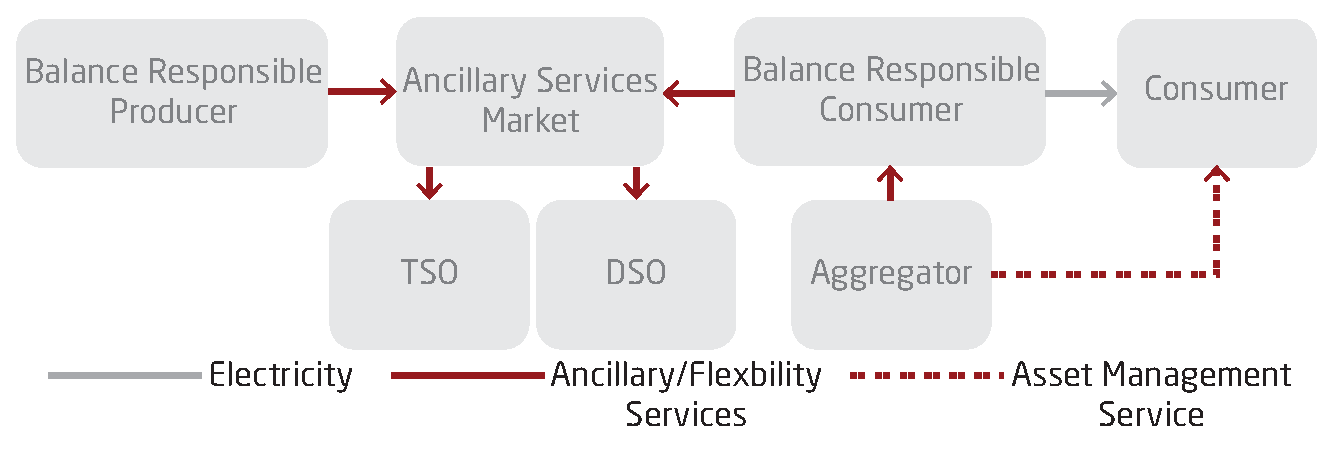
\includegraphics[width=\columnwidth]{graphics/tsg/market_future4}
  \caption{The new player in the market for ancillary services is the aggregator, which sells consumption flexibility on the ancillary service markets through the Balance Responsible Consumer. Some markets allow the aggregators to participate directly in the ancillary service markets with the condition that they coordinate with their Balance Responsible Consumer. It also provides flexibility services to BRPs and DSOs.}
  \label{fig:TSGmarket}
\end{figure}
%The aggregator will sign contracts with the DER owners and be the responsible party for delivery of service to the TSO, DSO or BRP. Further, the aggregator will have to ensure that certain performance parameters are respected towards the DER owner \cite{ding2013development}.
%Introduction of FLECH. \newline

\subsection{Service verification today}
When contracted for service, units are subject to a set of requirements. First, units must pass a prequalification test.% In PJM, when contracted for regulation, this consists of passing three consecutive tests.
Second, certified metering instrumentation must be installed on the unit, and telemetry equipment must be installed and connected to the system operator's Supervisory and Control Data Acquisition (SCADA) system.

For verifying reserve services, the system operator does random checks to see if the reserve is available at the unit \cite{EnerginetAncillary}. %\bondy{I'm not sure who to cite here... in ENDK AS document it is written that ENDK has the right to do random function checks, and that at any moment ENDK can ask for documentation of delivered service... but I've only had it from word of mouth that they actually sometimes do those random tests}\kh{but that's perfect - it's written that they can do it.}
With respect to regulation services, these are expected to be delivered within the required time requirements, and must be measured with acceptable accuracy. For example, for consumption units smaller than 1.5 MW acceptable accuracy is 2\% of the load \cite{Energinettek}.

%``service level agreements´´ etc.
%\kh{here should be a short outline of the actual service verification process; and how it's done today: pre-qualification, certified metering equipment on each generator , , then occasional (?) checks on the response; penalties for non-delivery, etc-}

\subsection{The need for service requirements modeling}\label{subsec:needforreq}
The concept of verification of ancillary services is moving towards a more flexible definition. Furthermore, new types of flexibility services are appearing, e.g. \cite{tougaard2015flech,heussen2013clearinghouse}. Part of the lessons learned from a demonstration of one of these new DSO services \cite{ipowerdemo,bondy2014powermax} is that the services, along with their requirements, need to be clearly defined if aggregators are to deliver them. The main problem being that the verification of services delivered by aggregators is complex.
%\hl{This is because it cannot be assumed that the services will be delivered by traditional (well understood) units, making verification more complex.} 
Also, research points at the need for change of the traditional service requirements if aggregators are to be enabled \cite{macdonald2012demand,koliou2014demand}. Thus, models that translate service contract requirements into benchmarks for performance assessment are needed.

From the market setup described in the previous section, parallels can be drawn to the concept of \emph{Service-Oriented Architectures} (SOAs) from the field of computer science. Under that paradigm, service is defined as: a logical representation of a repeatable business activity that has a specified outcome, is self-contained, may be composed of other services and is a \emph{black box} to consumers of the service \cite{opengroupsoa}. An element in SOAs are \emph{Standardized service contracts}, which contain service level agreements (SLAs). The SLAs can be interpreted as the requirements defined in an ancillary service contract. SLAs must define service performance metrics with corresponding service level objectives (SLOs), which are the agreed means for measuring performance.
%\kh{here motivate the need for formalized and generic requirements; good to use the iPower experience here as motivation}

PJM has established precedence in using performance metrics for verification of services. Their \emph{performance score} consists of a weighted average of three measures: delay, accuracy and precision. These measure the delay and correlation between the regulation signal and the reaction of the unit, and the difference in energy requested vs. energy supplied \cite{pjmperf}. These measures are tailored to the way frequency regulation is done at PJM (tracking of the regulation signal). Therefore, more general (and simple) models and performance metrics are needed to cover other frequency regulation services and the new flexibility services.

\section{Requirements and proposed test  procedure}\label{sec:metrics}
%\hl{- What alternative method do we propose?}

The objective of the current tests is to validate the parameters of a well understood model of generation units. For the reasons stated previously, the new tests need to identify an empirical behavior model of an uncertain and diverse entity: the aggregator control architecture and unit portfolio. 

%This means that there is no single standard test, but 
A test procedure is required that will allow the system operators to understand and predict the performance of a specific aggregator under a given set of operation conditions (Fig.~\ref{fig:framework}). In this section we present the underlying assumptions for such a procedure, the metrics used to measure the aggregator performance, and the proposed procedure.
%Getting an empirical model of an unknown entity rather than a mathematical model of a known entity. System identification approach.

\begin{figure}[!t]
\centering
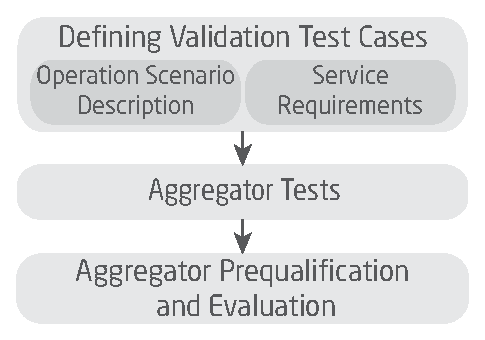
\includegraphics[width=1.7in]{graphics/pscc2016/validation.eps}
\caption{Schematic procedure for aggregator validation. The focus of this paper is on the relationship between the service requirements and the aggregator tests.}
\label{fig:framework}
\end{figure}

%Here the following three topics must be discussed:
%\begin{itemize}
%\item Boundary conditions (grid, DER)
%\item Fault scenarios
%\item Operation spectrum (what is the possibility/range of the input data?)
%\item Experimental design
%\end{itemize}

%The experiments should be able to measure response/states that can't be measured safely/easily under deployment.

%The tests must have a well defined input and output.

\subsection{Test Procedure Assumptions}\label{subsec:assumptions}
%A great variety of aggregator architectures has been proposed and implemented; differences between them are linked to specific business cases, local regulations, grid codes etc. Implementation details such as algorithms for portfolio composition, resource prediction or trading, constitute key intellectual property of commercially operating aggregators and disclosure of these business secrets will be unacceptable in many cases. For this reason,
The critical assumption are:

1) A general test design must start from the assumption that the aggregator and its infrastructure are to be treated as a black box, in the sense that only the aggregator inputs and outputs are known but the details of the internal control architecture are unknown.

%Field tests have been carried out in order to validate DR schemes, see e.g. \cite{kiliccote2013field}. While these kind of tests are important to characterize the capabilities of aggregators, the tests are not able to fully identify their operation capabilities. Thus, i
2) In order to fully test aggregators under a number of relevant scenarios, and to capture the stochastic nature of their operation, aggregators must be tested with the aid of a simulation framework. % While these kind of tests are important to characterize the capabilities of aggregators, the tests are not able to fully identify their operation capabilities.

3) It is assumed that such a simulation framework is detailed enough in terms of power system models, DER models and information and communication technology (ICT) systems in order for the simulation results to reflect the real performance of a deployed aggregator with sufficient precision.
%While a few tests are enough to ensure compliance of traditional generators, the stochastic nature of aggregators requires sufficient samples in order to capture the variance of the stochastic process that influences the aggregator performance. It is usually infeasible to subject a deployed and operational aggregator to a high number of tests, it is expected that aggregator validation must include simulation. In this way, the aggregator will be subjected to situations that are reproducible. 

The assumptions that can be adjusted are:

4) The tests are defined by a set of operational scenarios and service requirements (Fig.~\ref{fig:framework}): a) the operational scenarios define the statistical distribution of the test disturbances; b) the service requirements define the expected behavior of the aggregator. 

5) The mode of interaction between the test cases and the aggregator is defined in a test setup (Fig.~\ref{fig:test_setup}), where the disturbances (test inputs) defined in the operational scenarios affect the aggregator interaction with the DERs and the power grid. 

6) The aggregator has two interfaces: \emph{inputs} in the form of measurements and service reference signals received from the system operators; \emph{outputs} in the form of control domain signals exchanged between the aggregator and the units in its portfolio.

7) The operational scenarios are not designed to cover aggregator operation under exceptional system conditions. This means that the aggregator will not be held accountable for non-delivery in cases where the cause is outside of the aggregator's influence, e.g. in the case of grid faults. If communication between the aggregator and the controlled units, or internally within the aggregator architecture, occurs over public telecommunication networks, the robustness to network outages must be tested, for example by simulating disturbances and delays.

8) The flexibility which the aggregator can offer is bounded by the contractual requirements between the aggregator and its clients.

9) Aggregator validation will be carried out by a third party test entity.

\begin{figure}[!t]
\centering
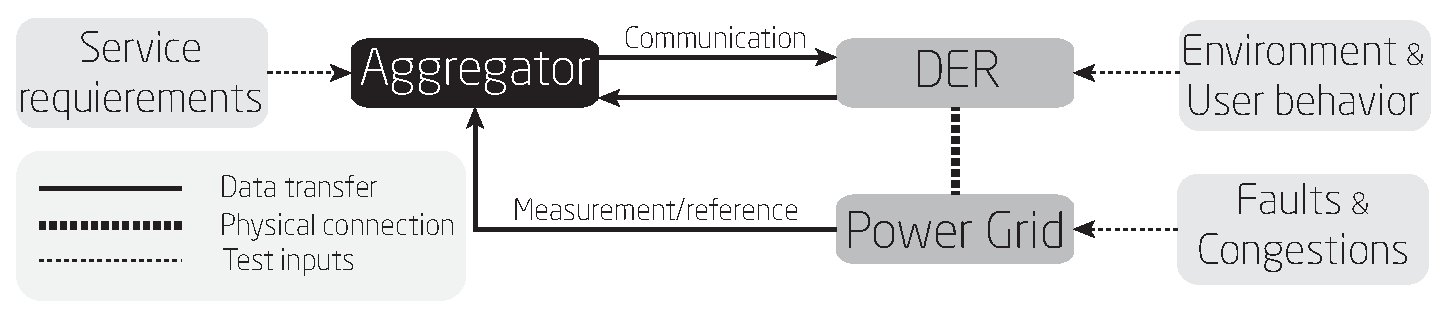
\includegraphics[width=\columnwidth]{graphics/pscc2016/test_setup.eps}
\caption{Schematic test setup where the test subject, the aggregator, is treated as a black box.}
\label{fig:test_setup}
\end{figure}

\subsection{Service Requirements - Test Metrics}\label{sec:servreqmet}

In order to measure how the disturbances affect service delivery, a set of service performance metrics must be established. The main purpose of the current tests is to verify communication, responsiveness to frequency changes and tracking of a reference or AGC\footnote{Automatic Generation Control, see e.g.\cite{entso1operational}.} signal. Coupling this with the performance requirements defined by the TSOs (e.g. \cite{energinet2012ancillary,ipower2013development}), the expected behavior of the considered services was analyzed (Table~\ref{tab:servmet}), and a set of requirement metrics were defined:
\begin{itemize}
\item Time responsiveness, i.e. how fast can the service be delivered from the moment the reference or measurement signal changes.
\item Grid responsiveness, i.e. how well can the aggregator follow changes in the grid state (marked with $\star$ where relevant on Tab.~\ref{tab:servmet}).
\item Response accuracy, i.e. how good is the aggregator in providing the full volume that is requested.
\end{itemize}


\begin{table}[!t]%% increase table row spacing, adjust to taste
\renewcommand{\arraystretch}{1.30}
% if using array.sty, it might be a good idea to tweak the value of
% \extrarowheight as needed to properly center the text within the cells
\caption{System services and their behavior}
\label{tab:servmet}
\centering
% Some packages, such as MDW tools, offer better commands for making tables
% than the plain LaTeX2e tabular which is used here.
\begin{tabularx}{\columnwidth}{p{1.0cm} X X}
\toprule
System Operator& Service name & Service behavior\\
\midrule
TSO & Frequency containment reserve (FCR) & autonomous response to frequency deviations ($\star$) \\
TSO & Frequency restoration reserve (FRR) & tracking of the AGC-signal\\
DSO & Congestion management         & reference tracking \\
    &                               & respecting a maximum feeder/transformer limit ($\star$) \\
    &                               & demand response \\
    &                               & grid state responsiveness ($\star$)\\
\bottomrule
\end{tabularx}
\end{table}

These three metrics will constitute the measure with which an aggregator will be deemed to perform according to service requirements, and the tests must excite the aggregator such that it is possible to determine through the value of these metrics the performance of the aggregator. It must be pointed out that the grid responsiveness metric is only applicable to the evaluation of aggregators providing services that rely on direct measurement of the grid, e.g. FCR.

When system operators define the acceptable values of the service requirement metrics, the values should have a statistical component. An example could be that the time responsiveness of a service provision should in average of 5 seconds, with a variance of $\pm$ 1 second. The actual indices used for the proposed metrics are discussed in Sec.\ref{sec:evaluation}.

\subsection{Aggregator Validation Procedure}\label{sec:alignment}
The procedure for aggregator validation applies statistical principles for the evaluation of the aggregator performance. It consists of the following steps:
\begin{enumerate}
	\item The general composition of the aggregator is established through documentation, and the service the aggregator is to be validated for is selected. %The aggregator informs of the general composition of its portfolio, as well as the service it wants to be validated for.
	\item The testing entity identifies the appropriate service requirements for the selected service.
	\item The testing entity identifies the expected normal operation of the aggregator based upon the service definition.
	\item The testing entity defines the operation scenarios that the aggregator is expected to perform under. %The scenarios must define the statistical properties, e.g. mean and variance, for the stochastic disturbances affecting the aggregator performance.
	\item The tests are carried out on the aggregator.
	\item The aggregator performance is evaluated.
\end{enumerate}

From the services analysed in this work, the tests are divided into two categories depending on their excitation signal:
\begin{itemize}
\item step response (like those for FCR),
\item continuous reference tracking (like those for FRR).
\end{itemize}

The validation tests will use one of these excitation signals under a different set of circumstances defined in the operation scenarios. Sufficient sampling of the aggregator response to the excitation signal is important in order to ensure that the mean and variance of the performance metrics give a realistic impression of the aggregator performance under deployment.%Thus, we formulate the following heuristic for the alignment of service requirements and tests: if a service
%The tests will evaluate the sensitivity of the aggregator to changes in the portfolio, and issues with the communication.


%\hl{The test procedure should be described. 2 diagrams are needed: 1st. shows the aggregator under normal operation (physical connection and the ICT connection), with relevant inputs and outputs of the aggregator. 2nd is the test process, where at each stage inputs are added/modified.}

% At the same time, based upon these two inputs, the overall service delivery is verified and evaluated, which is reflected in the bottom box of Figure~\ref{fig:framework}. \hl{Generally, I think we're still talking too much about the overall process and not about what the paper claims it's focusing on ("[...] the alignment of service requirements with the testing [...]"). On the latter we're not specific enough wrt what kind of result the reader can expect.}

%An aggregator infrastructure and control process is usually complex and therefore interactions of an aggregator may be tested separately. Depending on the metrics by which the relations are measured (Table~\ref{tab:metrics}), it is possible to test certain components through simulation or co-simulation, while other interactions require hardware-in-the-loop tests. This paper will propose a method for identifying the relationships between metric types and the tests necessary  for validating the measured function. The method will then be applied to several existing aggregator architectures as a proof of concept.

\subsection{Evaluation of Test Results}\label{sec:evaluation}
The service requirement metrics (Sec.~\ref{sec:servreqmet}) define the measure upon which the aggregator is evaluated. Different options exist that can be used to measure these metrics. One option is the aggregator performance index \cite{bondy2014performance}, which measures the error in service delivery for the services delivered to the system operators and the serviced delivered to the owners of the DERs. This metric captures both time responsiveness and response accuracy into a single value. A large set of performance indices exist within the field of control performance assessment, these can be utilised for the proposed validation method, see e.g. \cite{jelali2006overview}.

Given the stochastic nature of the tests, the indices will also be stochastic. The value of the performance indices is estimated at each iteration of the test, which means that the final value of the performance index reflects the stochasticity of the disturbances. For example, if the disturbances defined in the operation scenarios are Gaussian, the performance index will also have a mean and variance. These values need to be compared to those values defined in the service requirements. It will be the choice of the system operators what the service requirements should be, taking into consideration their risk adversity. Requiring a small variance on the performance indices minimizes the risk of not getting a full service delivery, but might also lead to more expensive services.


%\input{content/assumptions.tex}
\section{Case Study of the Validation Procedure }\label{sec:casestudy}

In this section we apply the concepts outlined in Sec.~\ref{sec:metrics} on a simplified example of the validation procedure on an aggregator architecture similar to the one presented in \cite{thavlov2013aggregation}. While the design of these operating scenarios is outside the scope of this paper, some overall assumptions have been made. The sample aggregator name is  DTU-FlexServices, and it wants to sell ancillary services to the TSO called RisøGrid. The validation tests are carried out by the independent company AggTesters. The rest of this section presents the reference scenario, the example of the aggregator test and the evaluation process. 

\subsection{Aggregator Framework \& Portfolio}
The objective of the DTU-FlexServices is to allocate a given amount of power, provided as a setpoint by the TSO, over a controllable portfolio of 100 resistive heating systems, each providing space heating to a detached household. The objective is subject to constraints on nominal power of the heating systems and indoor comfort, which is implemented as a tolerable band in which the temperature is allowed to vary given by the interval $\left[T_{min},T_{max}\right]$. It is assumed that feedback on measured indoor temperature is available to the aggregator, such that the aggregator in real-time can assess the available capacity of the controlled heating system and ensure that indoor temperature constraints are not being violated during operation. Fig. \ref{fig:flow_diagram} presents the flow of data in the aggregator simulation framework. 
\begin{figure}[!t]
\centering
\includegraphics[width=\columnwidth]{graphics/pscc2016/flowchart.eps}
\caption{Flow diagram of the aggregator algorithm.}
\label{fig:flow_diagram}
\end{figure}
The aggregator uses a simple auto-regressive model with exogenous inputs (ARX) to assess the future available capacity of each individual households. The ARX model is given by,
\begin{equation}\label{eq:capacity}
  T_{i+1} - a\cdot T_i = b \cdot T_{a,i} + c \cdot \Phi_{s,i} + \boldsymbol{d}^T \boldsymbol{\Phi}_{h,i:i-\tau_{lag}}
\end{equation} 
where $T_i$ is the measured indoor temperature of the household at time step $i$, $T_a$ is the outdoor temperature, $\Phi_s$ is the solar irradiance and $\boldsymbol{\Phi}_{h,i:i-\tau_{lag}}$ is a vector with the most recent observed power consumptions, i.e. $\left[\Phi_{h,i},\Phi_{h,i-1} \cdots \Phi_{h,i-\tau_{lag}}\right]$. The lag parameter of the heat input, $\tau_{lag}\in\mathbb{N}_0$, is used to account for the potential time-lag that might exists between when heating is applied and when it is observed in the indoor temperature. $a$, $b$, $c\in\mathbb{R}$, and $\boldsymbol{d}\in\mathbb{R}^{\tau_{lag}+1}$ are the unknown parameters of the ARX model, which are found using prior data for power consumption of the heating system. For simplicity $\tau\equiv 0$ is assumed in the following. 

Each individual resistive heating system is assumed to be able to dispatch a continuous amount of power in the interval $\left[P_{min}, P_{max}\right]$, given by the nominal power of the heating system. Naturally, this is an approximation since resistive heating systems, in general, will only be able to dispatch power in discrete steps due the composition of resistive loads. However, considering a portfolio of many entities and following the law of large numbers, these discrete steps should level out and the assumption hold. 

To allocate the amount of power over the portfolio of resistive heating system, following unit commitment problem is formulated,
\begin{align}\label{eq:agg_dispatch}
  & \min\;\left|\; \sum_{j=1}^N \left(\Phi_{h,i,j}\right) - S_i \;\right|\; + \; \sum^{N}_{j=1}\Phi_{h,i,j}\mbox{W}\left(T_{i+1,j}\right)	\\[5mm]\nonumber
  & \mbox{s.t.} \quad P_{min,j} \leq \Phi_{h,i,j} \leq P_{max,j}  
\end{align}
where the decision variable  $\Phi_{h,i,j}\in\mathbb{R}$ is the amount of power being allocated to household $j$ at time step $i$, $N$ is the number of households in the portfolio, $S_i$ is the setpoint given to the aggregator and $\mbox{W}\left(T_{i+1,j}\right)$ is a weight function of the predicted indoor temperature found from Equation \eqref{eq:capacity}. The weight function should be constructed such that $\mbox{W}\left(\cdot\right)<-1$ for $T_{i+1,j} < T_{min}$, thus making the last term dominate the cost function and force the allocated power up for household $j$. Likewise, $\mbox{W}\left(\cdot\right)>1$ for $T_{i+1,j} > T_{max}$, thus forcing the power down. Following linear weight-function is proposed,
\begin{equation}\label{eq:weight_fct}
  \mbox{W}\left(T_{i+1,j}\right) = \frac{2\left(T_{i+1,j}-T_{min,j} \right)}{T_{max,j} - T_{min,j}}-1 
\end{equation}
The simulation model of the individual households is implemented as a stochastic linear state space model in discrete time, which is     given by
\begin{align}\label{eq:simulation_model}
  \boldsymbol{T}_{i+1} &= \boldsymbol{A}\boldsymbol{T}_i + \boldsymbol{B}\boldsymbol{U} + \boldsymbol{\sigma}_i \\\nonumber
  T_i &= \boldsymbol{C}\boldsymbol{T} + e_i
\end{align}
where $T_i\in\mathbb{R}$ is the locally measured indoor temperature which is assumed to be forwarded to the aggregator, $\boldsymbol{T}_i\in\mathbb{R}^n$ is the state vector and $\boldsymbol{U}\in\mathbb{R}^m$ is the input vector. $\boldsymbol{A}\in\mathbb{R}^{n\times n}$, $\boldsymbol{B}\in\mathbb{R}^{n\times m}$ and $\boldsymbol{C}\in\mathbb{R}^{1\times m}$ are the system, input and output matrix, respectively. To account for unrecognized input and approximations, process noise, $\boldsymbol{\sigma}_i\in\mathbb{R}^n$, is added to the system equation, \eqref{eq:simulation_model}. In the following, $\boldsymbol{\sigma}$ is assumed to be a Gaussian white noise process. Furthermore, $n\equiv1$ is assumed, i.e. only one temperature state is being simulated in the households; hence, since a Gaussian white noise process is fully characterized by its variance, the process noise is fully described by the variance $\sigma\in\mathbb{R}$.% Naturally, a single state would not be sufficient for thermally heavy households with multiple heat reservoirs, e.g. households with floor heating.

The aggregator framework and simulation models, simulating the considered scenario, have been implemented in \textsc{matlab} and is presented in full detail in \cite{thavlov2013aggregation}. It is important to note that the aggregator is described in this section for the purpose of the paper, but this description is contained within the conceptual black box described in Sec.~\ref{subsec:assumptions}, and the testing entity only has access to the general composition of the aggregator portfolio.

\subsection{Service Requirements, Normal Operation and Operation Scenario}\label{subsec:scenario}
The DTU-FlexServices aggregator wants to participate in the ancillary service markets with a FRR up-regulation service with a volume of 250 kW. 
Since it is the first time DTU-FlexServices participates in the market for this service, RisøGrid requires DTU-FlexServices to go through the validation process. Following the steps outlined in Sec.~\ref{sec:alignment}, the validation process consists of the following steps:
\begin{enumerate}
\item DTU-FlexServices presents the documentation for its portfolio.
\item RisøGrid sets the test service requirements as:
    \begin{itemize}
        \item Response accuracy:  $E[RMS] \leq 60\,kW$
        \item The response durations: $\tau = 1\,h$
    \end{itemize}
\item AggTesters identifies the normal operation scenario as:
    \begin{itemize}
        \item One source of uncertainty is the availability of the portfolio, which is a uniform distribution between 70\% and 100\%. This also accounts for minor changes in the portfolio size.
        \item A second source of uncertainty is in the disturbances induced by unrecognized user behavior and inaccurate weather forecast in the house simulation model. This uncertainty is described by $\sigma$ in Eq.~\eqref{eq:simulation_model}.
    \end{itemize}
\end{enumerate}

\subsection{Aggregator test}
To test for different combinations of the two sources of uncertainties, a series of simulations are carried out with permutations of the two. Assuming the availability to be uniformly distributed, the tests are carried out in discrete steeps across the 70\% -- 100\% spectrum of availability. Likewise, the variance of the noise process is tested in discrete steps in the 0.00 -- 0.30 domain. Fig.~\ref{fig:test100} and Fig.~\ref{fig:test70} present the outcome of two different simulations for 100\% and 70\% availability, respectively, and $\sigma=0.10$. Each permutation of the two noise sources is simulated 100 times.
\begin{figure}[!t]
%\centerline{
\centering
\subfloat[Response accuracy]{\includegraphics[width=0.85\columnwidth]{graphics/pscc2016/agg_power_ctrl_100SH_0STATIC_05PCT_REDUCTION.eps}%
\label{fig:ref100}}
%\vfill
\\
\subfloat[House Temperatures]{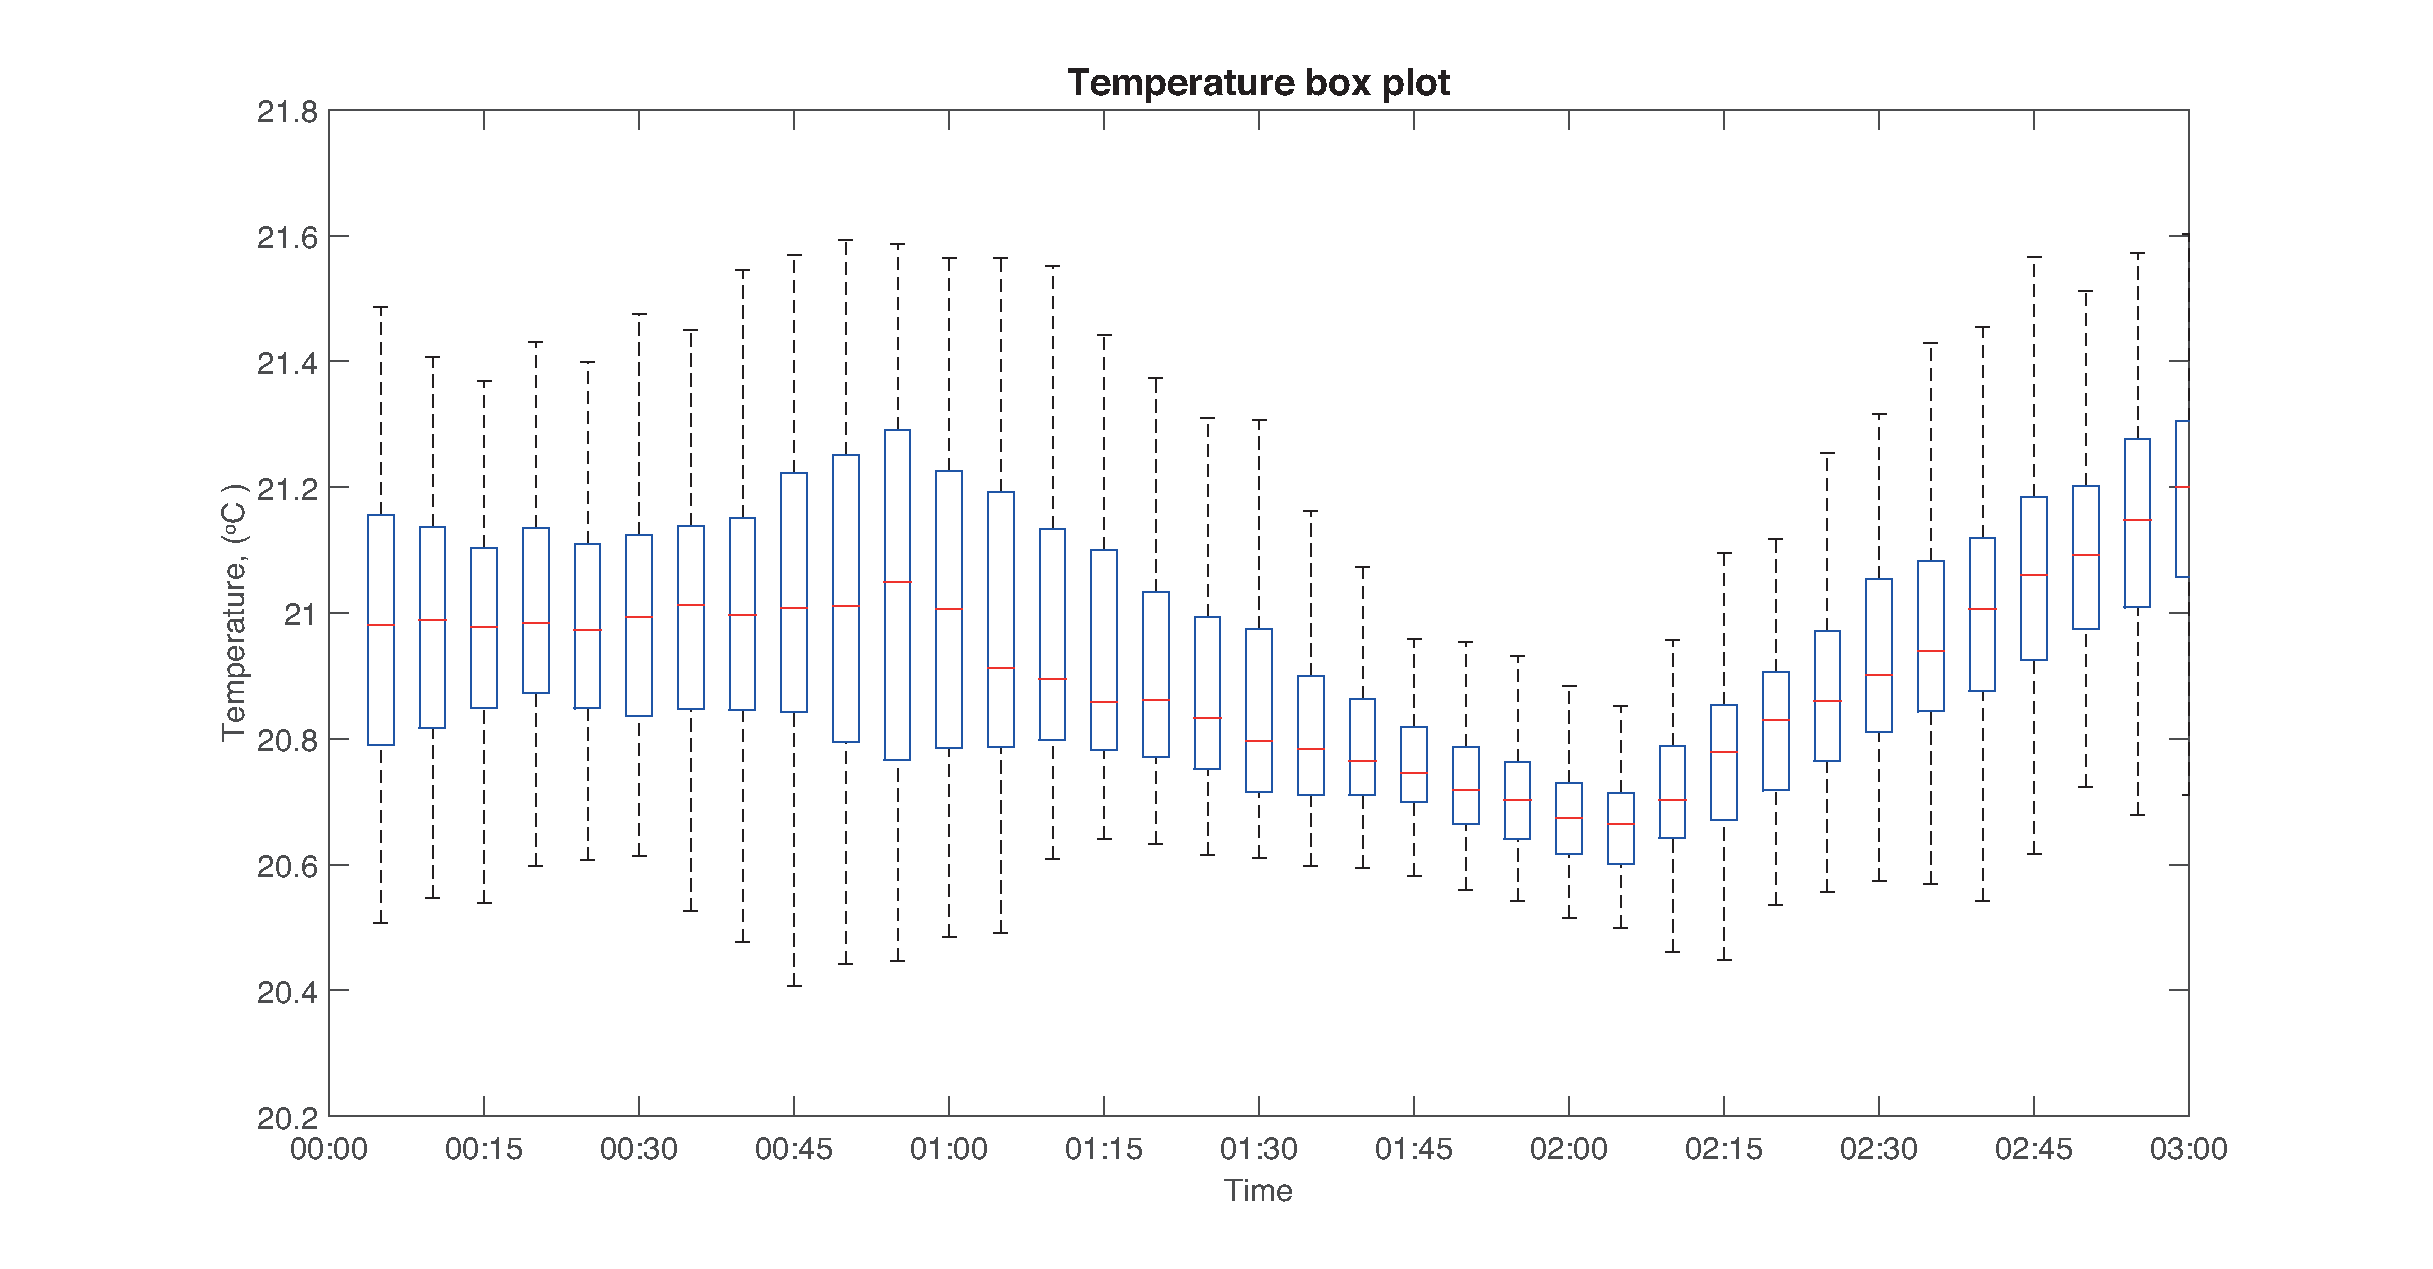
\includegraphics[width=\columnwidth]{graphics/pscc2016/agg_box_plot_100SH_0STATIC_05PCT_REDUCTION.eps}%
\label{fig:temp100}}%}
\caption{Simulation results of the 100\% availability test for the whole portfolio.}
\label{fig:test100}
\end{figure}

\begin{figure}[!t]
%\centerline{
\centering
\subfloat[Response accuracy]{\includegraphics[width=0.85\columnwidth]{graphics/pscc2016/agg_power_ctrl_70SH_30STATIC_05PCT_REDUCTION.eps}%
\label{fig:ref70}}
%\vfill
\\
\subfloat[House Temperatures]{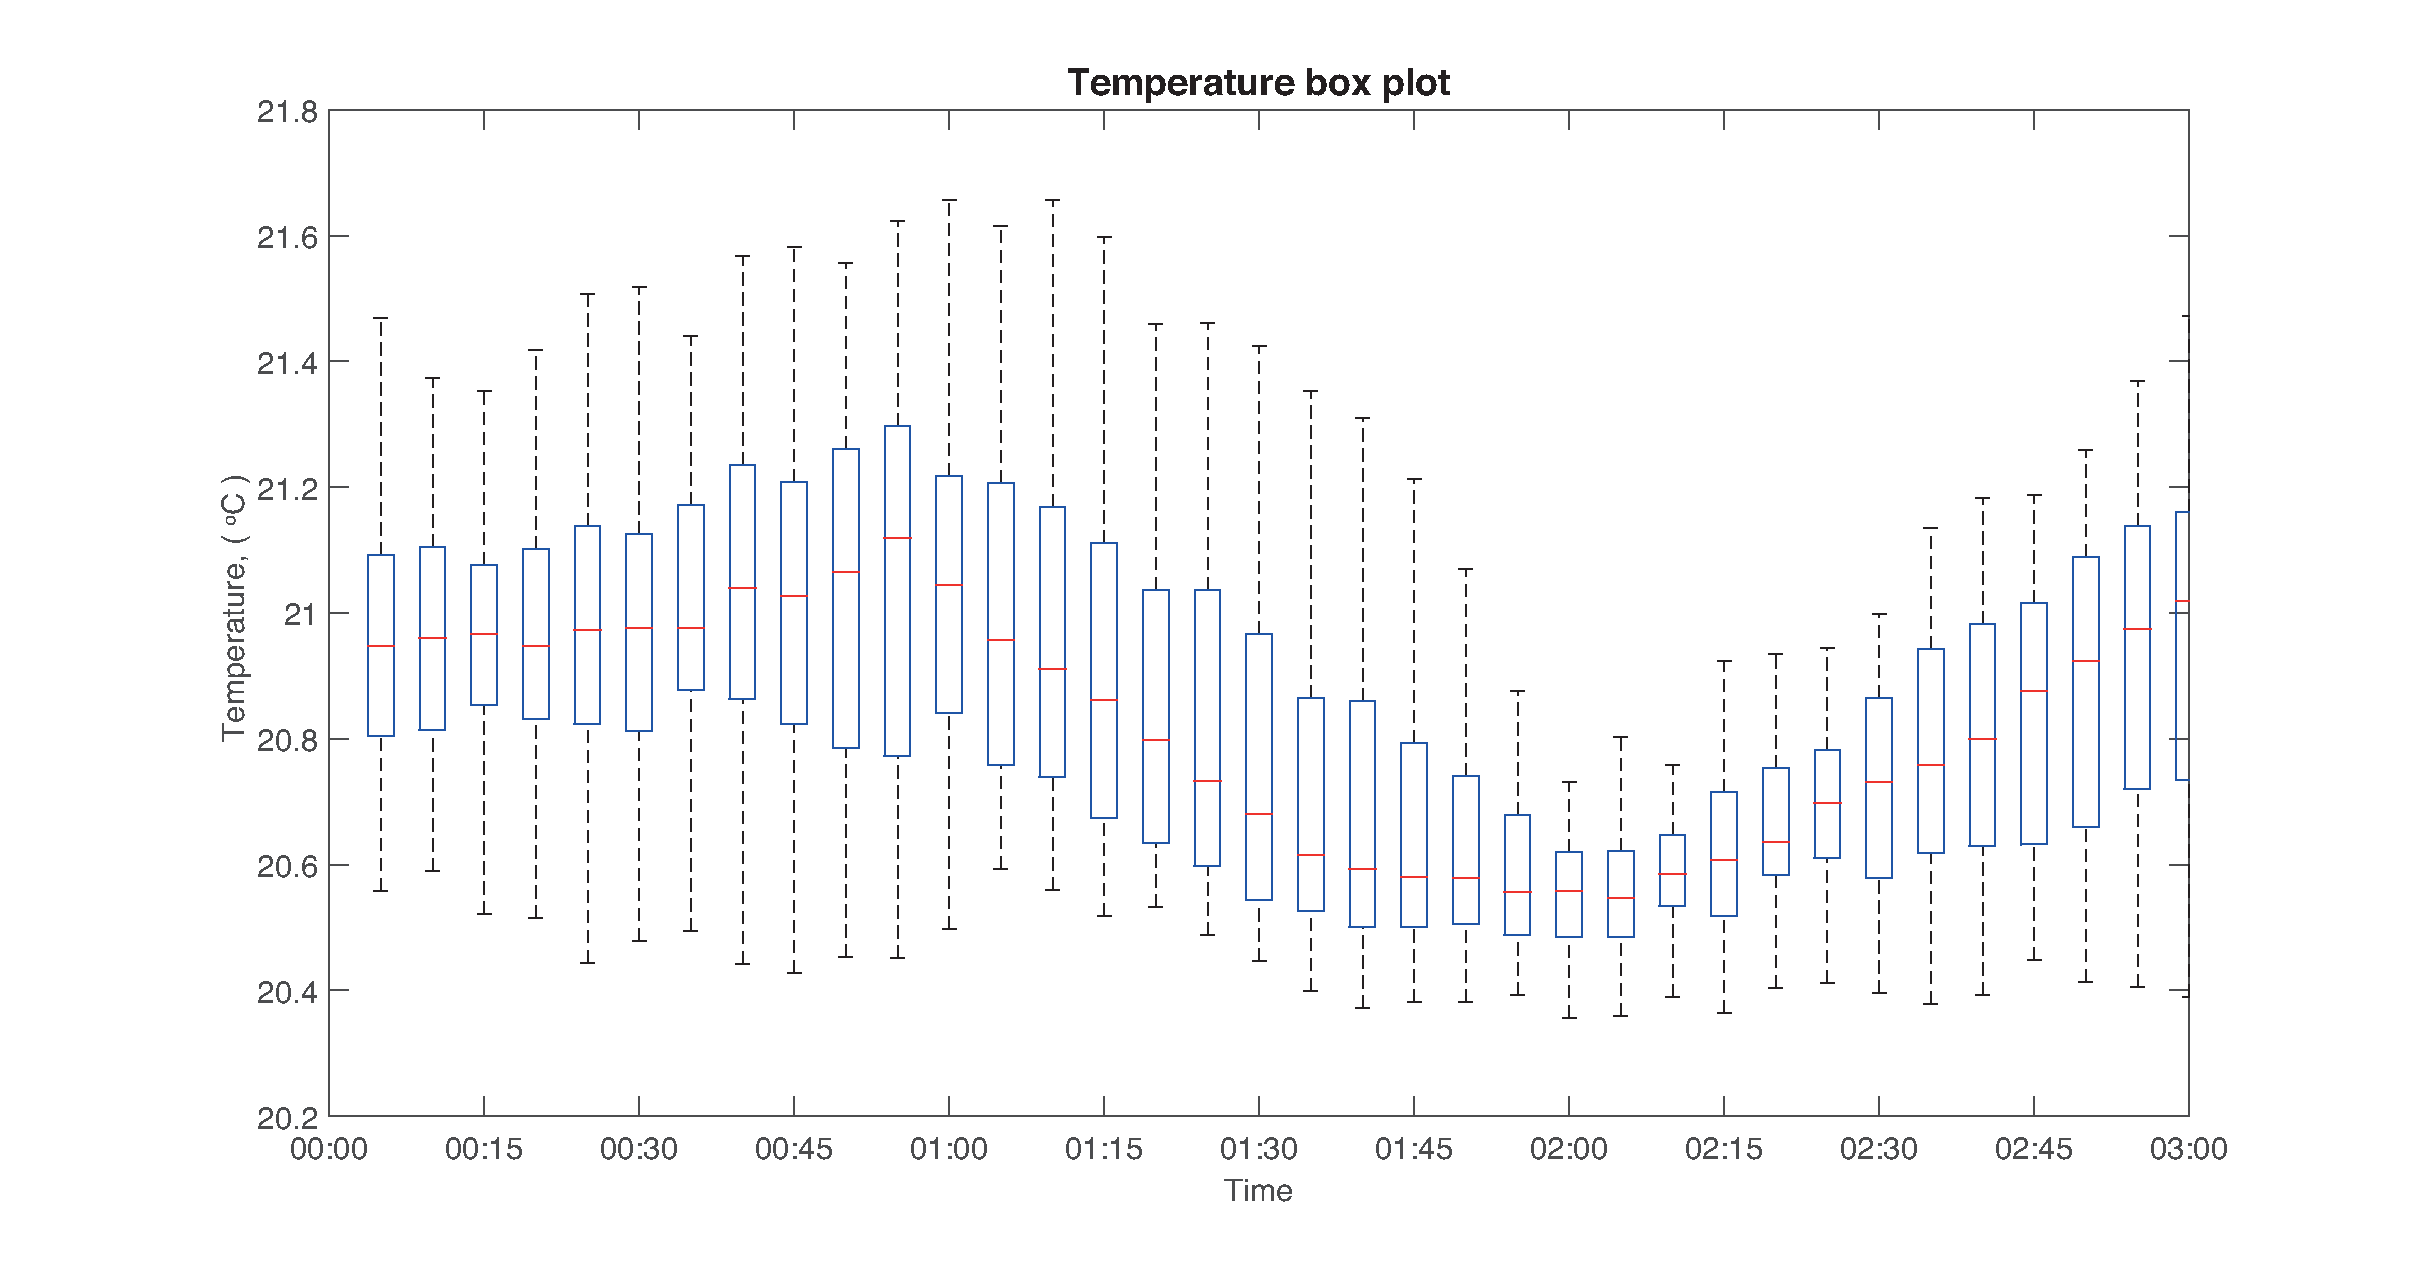
\includegraphics[width=\columnwidth]{graphics/pscc2016/agg_box_plot_70SH_30STATIC_05PCT_REDUCTION.eps}%
\label{fig:temp70}}%}
\caption{Simulation results of the 70\% availability test for the whole portfolio}
\label{fig:test70}
\end{figure}

The response accuracy of DTU-FlexServices and the average temperature of its portfolio can be seen in Fig.~\ref{fig:ref100} and Fig.~\ref{fig:ref70}. The distribution of the house temperatures can be seen in Fig.~\ref{fig:temp100} and Fig.~\ref{fig:temp70}, and it is clear that as the availability of the houses decreases, the flexibility for up-regulation is being saturated faster and the DTU-FlexServices is unable to track the FRR reference signal.

Having carried out the necessary test, RisøGrid proceeds to evaluate the results of the tests.

\subsection{Evaluation of test results}
Since the case study looks at simplified setup, and the example does not take the time responsiveness metric into account, it does not make sense to use the aggregator performance metric mentioned in Sec.~\ref{sec:evaluation}. In Sec~\ref{subsec:scenario}, the root mean square (RMS) error is chosen to measure the response accuracy metric: 
\begin{equation}
  \eta_{RMS} = \sqrt{\frac{1}{M}\sum_{i=1}^M\left(\sum_{j=1}^N\left(\Phi_{h,i,j}\right) - S_i\right)^2}
\end{equation}
where $\left[1,M\right]$ are the iterations where the aggregator has been activated. The results of the test are presented in Table~\ref{tab:results}, where it can be seen that $E[\eta_{RMS}]<60 \, kW$. Therefore the DTU-FlexServices is certified to provide FRR up-regulation service to RisøGrid.
\begingroup
\setlength{\tabcolsep}{4pt}%
\begin{table}[!t]%% increase table row spacing, adjust to taste
\renewcommand{\arraystretch}{0.9}
% if using array.sty, it might be a good idea to tweak the value of
% \extrarowheight as needed to properly center the text within the cells
\caption{Performance of DTU-FlexServices}
\label{tab:results}
\centering
% Some packages, such as MDW tools, offer better commands for making tables
% than the plain LaTeX2e tabular which is used here.
\begin{tabular}{clcccccccc}
\toprule
        & & \multicolumn{7}{c}{Process noise, $\sigma$}                   & Avg. \\
        & & 0.00   & 0.05   & 0.10   & 0.15   & 0.20   & 0.25    & 0.30   &         \\ 
\midrule
\multirow{7}{*}{\rotatebox[origin=c]{90}{Availability}} 
& 100\%   & 0.00   & 0.00   & 0.04   & 9.25   & 31.20  & 48.84   & 98.32  & 26.81   \\
& 95\%    & 0.03   & 0.00   & 1.51   & 19.19  & 37.97  & 66.56   & 102.05 & 32.47   \\
& 90\%    & 1.40   & 0.04   & 14.36  & 30.78  & 58.74  & 73.38   & 98.24  & 39.56   \\
& 85\%    & 1.10   & 35.23  & 4.06   & 45.28  & 83.06  & 83.40   & 115.11 & 52.46   \\
& 80\%    & 13.88  & 29.25  & 12.94  & 65.93  & 72.31  & 94.50   & 135.85 & 60.67   \\
& 75\%    & 54.28  & 40.74  & 39.91  & 75.22  & 86.14  & 114.13  & 135.76 & 78.03   \\
& 70\%    & 45.63  & 90.90  & 85.41  & 99.02  & 93.68  & 123.82  & 142.64 & 97.30   \\
\midrule
Avg. & & 16.62  & 28.02  & 22.60  & 49.24  & 66.16  & 86.38   & 118.28 & 55.33   \\
\bottomrule
\end{tabular}
\end{table}
\endgroup
%\begin{figure}[!t]
%\centering
%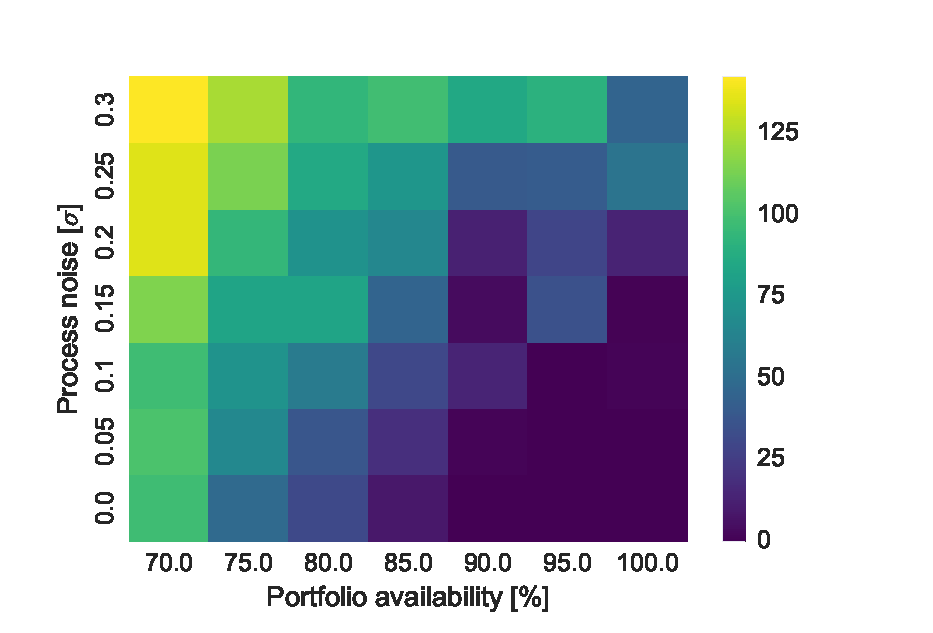
\includegraphics[width=\columnwidth]{figures/heatmap.eps}
%\caption{The RMS value over the test space. It can be seen that it is more important to have certainty in the portfolio availability than in the process noise.}
%\label{fig:colormap}
%\end{figure}

%\section{Quality Metrics}

What aspects of the aggregator influence in the performance metrics?

Internal vs. external metrics: external can be used for monitoring, internal can only manipulated in test environment.

Are there more metrics than in the table? E.g. robustness toward grid faults

\begin{table}[!t]%% increase table row spacing, adjust to taste
\renewcommand{\arraystretch}{1.3}
% if using array.sty, it might be a good idea to tweak the value of
% \extrarowheight as needed to properly center the text within the cells
\caption{System interactions can be evaluated with generalized metrics}
\label{tab:metrics}
\centering
% Some packages, such as MDW tools, offer better commands for making tables
% than the plain LaTeX2e tabular which is used here.
\begin{tabular}{ll}
\toprule
System interaction & metrics\\
\midrule
Aggregator - power system & responsiveness w.r.t. grid conditions\\
\\
Aggregator - DER portfolio & responsiveness w.r.t. time\\
 & robustness w.r.t. forecast errors\\
 \\
Aggregator -  ICT infrastructure & robustness w.r.t. communication faults\\
\bottomrule
\end{tabular}
\end{table}

\begin{table}[!t]
\renewcommand{\arraystretch}{1.3}
\caption{The quality metrics can be separated into two categories.}
\label{tab:metricsclass}
\centering
\begin{tabular}{ll}
\toprule
External metrics & Internal metrics\\
\midrule
responsiveness w.r.t. grid &robustness w.r.t. forecast errors\\
responsiveness w.r.t. time & robustness w.r.t. communication errors\\
& robustness w.r.t. grid errors\\
\bottomrule
\end{tabular}
\end{table}
\section{Conclusion and Future Work}
This work presents an initial approach to establishing a methodology for designing aggregator validation tests. This method differs from the traditional generator certification tests in that it must be carried out in simulations, so that the stochasticity of the real world disturbances affecting the aggregator can be taken into account. A drawback of this method is that it relies on the accuracy and complexity of the simulation models. This means that the components of the validation tests must be validated against reality. The test method was shown through a simplified case study on an existing aggregator. While the example shows a fictive TSO applying the test to a fictive aggregator, there is the possibility that validation of aggregators in the future will be carried out by third party test companies. 

There are still several open issues that need to be investigated with regards to aggregator validation. For example, the definition of the operation scenarios was only briefly discussed, and heuristics must be developed in order to define scenarios that are effective when testing aggregators.

An important step for the development of the validation method is the implementation of a complete test architecture with validated component models. With such a simulation framework, with realistic communication and DER models, communication delays can be implemented in order to test aggregators for time responsiveness. 

Finally, the method should be expanded to cover other ancillary services, such as voltage regulation.

We consider the work presented here an important element of enabling aggregators in the smart grid, thus enabling consumption to actively participate in the secure operation of the power system. This will help the integration of renewable energy sources into the power system.


%\section{Case Study}
%Here we present the validation process required for an aggregator developed at SYSLAB\cite{syslab}. \hl{Unless we're explaining what we're doing with SYSLAB, there isn't really much of a point in dropping the name here. This section should really talk about the expected results from the paper.}

%\section{Future Work}
% needed in second column of first page if using \IEEEpubid
%\IEEEpubidadjcol

% An example of a floating figure using the graphicx package.
% Note that \label must occur AFTER (or within) \caption.
% For figures, \caption should occur after the \includegraphics.
% Note that IEEEtran v1.7 and later has special internal code that
% is designed to preserve the operation of \label within \caption
% even when the captionsoff option is in effect. However, because
% of issues like this, it may be the safest practice to put all your
% \label just after \caption rather than within \caption{}.
%
% Reminder: the "draftcls" or "draftclsnofoot", not "draft", class
% option should be used if it is desired that the figures are to be
% displayed while in draft mode.
%
%\begin{figure}[!t]
%\centering
%\includegraphics[width=2.5in]{myfigure}
% where an .eps filename suffix will be assumed under latex, 
% and a .pdf suffix will be assumed for pdflatex; or what has been declared
% via \DeclareGraphicsExtensions.
%\caption{Simulation Results}
%\label{fig_sim}
%\end{figure}

% Note that IEEE typically puts floats only at the top, even when this
% results in a large percentage of a column being occupied by floats.


% An example of a double column floating figure using two subfigures.
% (The subfig.sty package must be loaded for this to work.)
% The subfigure \label commands are set within each subfloat command, the
% \label for the overall figure must come after \caption.
% \hfil must be used as a separator to get equal spacing.
% The subfigure.sty package works much the same way, except \subfigure is
% used instead of \subfloat.
%
%\begin{figure*}[!t]
%\centerline{\subfloat[Case I]\includegraphics[width=2.5in]{subfigcase1}%
%\label{fig_first_case}}
%\hfil
%\subfloat[Case II]{\includegraphics[width=2.5in]{subfigcase2}%
%\label{fig_second_case}}}
%\caption{Simulation results}
%\label{fig_sim}
%\end{figure*}
%
% Note that often IEEE papers with subfigures do not employ subfigure
% captions (using the optional argument to \subfloat), but instead will
% reference/describe all of them (a), (b), etc., within the main caption.


% An example of a floating table. Note that, for IEEE style tables, the 
% \caption command should come BEFORE the table. Table text will default to
% \footnotesize as IEEE normally uses this smaller font for tables.
% The \label must come after \caption as always.
%
%\begin{table}[!t]
%% increase table row spacing, adjust to taste
%\renewcommand{\arraystretch}{1.3}
% if using array.sty, it might be a good idea to tweak the value of
% \extrarowheight as needed to properly center the text within the cells
%\caption{An Example of a Table}
%\label{table_example}
%\centering
%% Some packages, such as MDW tools, offer better commands for making tables
%% than the plain LaTeX2e tabular which is used here.
%\begin{tabular}{|c||c|}
%\hline
%One & Two\\
%\hline
%Three & Four\\
%\hline
%\end{tabular}
%\end{table}


% Note that IEEE does not put floats in the very first column - or typically
% anywhere on the first page for that matter. Also, in-text middle ("here")
% positioning is not used. Most IEEE journals use top floats exclusively.
% Note that, LaTeX2e, unlike IEEE journals, places footnotes above bottom
% floats. This can be corrected via the \fnbelowfloat command of the
% stfloats package.








% if have a single appendix:
%\appendix[Proof of the Zonklar Equations]
% or
%\appendix  % for no appendix heading
% do not use \section anymore after \appendix, only \section*
% is possibly needed

% use appendices with more than one appendix
% then use \section to start each appendix
% you must declare a \section before using any
% \subsection or using \label (\appendices by itself
% starts a section numbered zero.)
%


% use section* for acknowledgement
%\section*{Acknowledgment}
%Parts of this work are supported by the Innovation Fund Denmark through the iPower project.



% Can use something like this to put references on a page
% by themselves when using endfloat and the captionsoff option.
\ifCLASSOPTIONcaptionsoff
  \newpage
\fi



% trigger a \newpage just before the given reference
% number - used to balance the columns on the last page
% adjust value as needed - may need to be readjusted if
% the document is modified later
%\IEEEtriggeratref{8}
% The "triggered" command can be changed if desired:
%\IEEEtriggercmd{\enlargethispage{-5in}}

% references section

% can use a bibliography generated by BibTeX as a .bbl file
% BibTeX documentation can be easily obtained at:
% http://www.ctan.org/tex-archive/biblio/bibtex/contrib/doc/
% The IEEEtran BibTeX style support page is at:
% http://www.michaelshell.org/tex/ieeetran/bibtex/
\bibliographystyle{IEEEtran}
% argument is your BibTeX string definitions and bibliography database(s)
%\bibliography{IEEEabrv,../bib/paper}
\bibliography{bib/references}
%
% <OR> manually copy in the resultant .bbl file
% set second argument of \begin to the number of references
% (used to reserve space for the reference number labels box)
%\begin{thebibliography}{1}
%
%\bibitem{IEEEhowto:kopka}
%H.~Kopka and P.~W. Daly, \emph{A Guide to \LaTeX}, 3rd~ed.\hskip 1em plus
%  0.5em minus 0.4em\relax Harlow, England: Addison-Wesley, 1999.
%
%\end{thebibliography}

% biography section
% 
% If you have an EPS/PDF photo (graphicx package needed) extra braces are
% needed around the contents of the optional argument to biography to prevent
% the LaTeX parser from getting confused when it sees the complicated
% \includegraphics command within an optional argument. (You could create
% your own custom macro containing the \includegraphics command to make things
% simpler here.)
%\begin{biography}[{\includegraphics[width=1in,height=1.25in,clip,keepaspectratio]{mshell}}]{Michael Shell}
% or if you just want to reserve a space for a photo:

%\begin{IEEEbiography}[{\includegraphics[width=1in,height=1.25in,clip,keepaspectratio]{picture}}]{John Doe}
%\blindtext
%\end{IEEEbiography}

% You can push biographies down or up by placing
% a \vfill before or after them. The appropriate
% use of \vfill depends on what kind of text is
% on the last page and whether or not the columns
% are being equalized.

%\vfill

% Can be used to pull up biographies so that the bottom of the last one
% is flush with the other column.
%\enlargethispage{-5in}




% that's all folks
\end{document}


